\documentclass[ngerman]{scrbook}
%%%%%%%%%%%%%%%%%%%%%%%%%%%%%%%%%%%%%%%%%%%%%%%%%%%%%%%%%%%%%%%%%%%%%%%%%%%%%%%
%%% Use option draft=true to enable markers in the text helping the author
%%% to find typographic errors
%%%
%%% Use draft=false for productive use, e. g. printing the document
%%%%%%%%%%%%%%%%%%%%%%%%%%%%%%%%%%%%%%%%%%%%%%%%%%%%%%%%%%%%%%%%%%%%%%%%%%%%%%%
\KOMAoptions{draft=true}

% Include LaTex packages
%%%%%%%%%%%%%%%%%%%%%%%%%%%%%%%%%%%%%%%%%%%%%%%%%%%%%%%%%%%%%%%%%%%%%%%%%%%%%%%
%%% Specify utf8 als input encoding. Usefull to be able to use 
%%% ä, ö, ü, ... directly
%%%
%%% http://ftp.uni-erlangen.de/ctan/macros/latex/base/inputenc.pdf
%%%%%%%%%%%%%%%%%%%%%%%%%%%%%%%%%%%%%%%%%%%%%%%%%%%%%%%%%%%%%%%%%%%%%%%%%%%%%%%
\usepackage[utf8]{inputenc}

%%%%%%%%%%%%%%%%%%%%%%%%%%%%%%%%%%%%%%%%%%%%%%%%%%%%%%%%%%%%%%%%%%%%%%%%%%%%%%%
%%% supports the Text Companion fonts, which provide many text symbols 
%%% 
%%% https://ctan.org/pkg/textcomp?lang=de
%%%%%%%%%%%%%%%%%%%%%%%%%%%%%%%%%%%%%%%%%%%%%%%%%%%%%%%%%%%%%%%%%%%%%%%%%%%%%%%
\usepackage{textcomp}

%%%%%%%%%%%%%%%%%%%%%%%%%%%%%%%%%%%%%%%%%%%%%%%%%%%%%%%%%%%%%%%%%%%%%%%%%%%%%%%
%%% defines Adobe Times Roman (or equivalent) as default text font
%%%
%%% https://ctan.mc1.root.project-creative.net/macros/latex/required/psnfss/psnfss2e.pdf
%%%%%%%%%%%%%%%%%%%%%%%%%%%%%%%%%%%%%%%%%%%%%%%%%%%%%%%%%%%%%%%%%%%%%%%%%%%%%%%
\usepackage{mathptmx}

%%%%%%%%%%%%%%%%%%%%%%%%%%%%%%%%%%%%%%%%%%%%%%%%%%%%%%%%%%%%%%%%%%%%%%%%%%%%%%%
%%% Select T1 as font encoding.
%%%%%%%%%%%%%%%%%%%%%%%%%%%%%%%%%%%%%%%%%%%%%%%%%%%%%%%%%%%%%%%%%%%%%%%%%%%%%%%
\usepackage[T1]{fontenc}

%%%%%%%%%%%%%%%%%%%%%%%%%%%%%%%%%%%%%%%%%%%%%%%%%%%%%%%%%%%%%%%%%%%%%%%%%%%%%%%
%%% Use new german orthography
%%%
%%% http://ctan.ebinger.cc/tex-archive/macros/latex/contrib/babel-contrib/german/ngermanb.pdf
%%%%%%%%%%%%%%%%%%%%%%%%%%%%%%%%%%%%%%%%%%%%%%%%%%%%%%%%%%%%%%%%%%%%%%%%%%%%%%%
\usepackage[ngerman]{babel}


%%%%%%%%%%%%%%%%%%%%%%%%%%%%%%%%%%%%%%%%%%%%%%%%%%%%%%%%%%%%%%%%%%%%%%%%%%%%%%%
%%% Provides support for setting the spacing between lines in a document
%%%%%%%%%%%%%%%%%%%%%%%%%%%%%%%%%%%%%%%%%%%%%%%%%%%%%%%%%%%%%%%%%%%%%%%%%%%%%%%
\usepackage[onehalfspacing]{setspace}

%%%%%%%%%%%%%%%%%%%%%%%%%%%%%%%%%%%%%%%%%%%%%%%%%%%%%%%%%%%%%%%%%%%%%%%%%%%%%%%
%%% Enables the user to define extended options when using graphics and figures
%%%
%%% http://ctan.ebinger.cc/tex-archive/macros/latex/contrib/babel-contrib/german/ngermanb.pdf
%%%%%%%%%%%%%%%%%%%%%%%%%%%%%%%%%%%%%%%%%%%%%%%%%%%%%%%%%%%%%%%%%%%%%%%%%%%%%%%
\usepackage[pdftex]{xcolor,graphicx}

%%%%%%%%%%%%%%%%%%%%%%%%%%%%%%%%%%%%%%%%%%%%%%%%%%%%%%%%%%%%%%%%%%%%%%%%%%%%%%%
%%% This package provides advanced facilities for inline and display quotations. 
%%%
%%% https://ftp.agdsn.de/pub/mirrors/latex/dante/macros/latex/contrib/csquotes/csquotes.pdf
%%%%%%%%%%%%%%%%%%%%%%%%%%%%%%%%%%%%%%%%%%%%%%%%%%%%%%%%%%%%%%%%%%%%%%%%%%%%%%%
\usepackage[babel,german=quotes]{csquotes}

%%%%%%%%%%%%%%%%%%%%%%%%%%%%%%%%%%%%%%%%%%%%%%%%%%%%%%%%%%%%%%%%%%%%%%%%%%%%%%%
%%% This package provides chapter pagenumbering style
%%%
%%% https://ftp.agdsn.de/pub/mirrors/latex/dante/macros/latex/contrib/chappg/chappg.pdf
%%%%%%%%%%%%%%%%%%%%%%%%%%%%%%%%%%%%%%%%%%%%%%%%%%%%%%%%%%%%%%%%%%%%%%%%%%%%%%%
\usepackage{chappg}


%%%%%%%%%%%%%%%%%%%%%%%%%%%%%%%%%%%%%%%%%%%%%%%%%%%%%%%%%%%%%%%%%%%%%%%%%%%%%%%
%%% allows you to add mini-tables-of-contents (minitocs) at the beginning of every chapter
%%%
%%% http://ctan.ebinger.cc/tex-archive/macros/latex/contrib/etoc/etoc-DE.pdf
%%%%%%%%%%%%%%%%%%%%%%%%%%%%%%%%%%%%%%%%%%%%%%%%%%%%%%%%%%%%%%%%%%%%%%%%%%%%%%%
\usepackage{etoc}

%%%%%%%%%%%%%%%%%%%%%%%%%%%%%%%%%%%%%%%%%%%%%%%%%%%%%%%%%%%%%%%%%%%%%%%%%%%%%%%
%%% KOMAScript guide, p. 271
%%%%%%%%%%%%%%%%%%%%%%%%%%%%%%%%%%%%%%%%%%%%%%%%%%%%%%%%%%%%%%%%%%%%%%%%%%%%%%%
\usepackage{scrlayer-scrpage}

%%%%%%%%%%%%%%%%%%%%%%%%%%%%%%%%%%%%%%%%%%%%%%%%%%%%%%%%%%%%%%%%%%%%%%%%%%%%%%%
%%% A macro package for creating graphics
%%%
%%% http://cremeronline.com/LaTeX/minimaltikz.pdf
%%%%%%%%%%%%%%%%%%%%%%%%%%%%%%%%%%%%%%%%%%%%%%%%%%%%%%%%%%%%%%%%%%%%%%%%%%%%%%%
\usepackage{tikz}

%%%%%%%%%%%%%%%%%%%%%%%%%%%%%%%%%%%%%%%%%%%%%%%%%%%%%%%%%%%%%%%%%%%%%%%%%%%%%%%
%%% Self defined library for emr diagrams
%%%
%%% https://github.com/harrisony/tikz-er2/tree/usyd/docs
%%%%%%%%%%%%%%%%%%%%%%%%%%%%%%%%%%%%%%%%%%%%%%%%%%%%%%%%%%%%%%%%%%%%%%%%%%%%%%%
\usepackage{tikz-er2}
  % Einstellungen fuer Tikz
  \usetikzlibrary{positioning}
  \usetikzlibrary{shadows}
  \usetikzlibrary{calc}
  \usetikzlibrary{arrows}
  \tikzstyle{every entity} = [top color=white, bottom color=blue!30,
                              draw=blue!50!black!100, drop shadow]
  \tikzstyle{every weak entity} = [drop shadow={shadow xshift=.7ex,
                                  shadow yshift=-.7ex}]
  \tikzstyle{every attribute} = [top color=white, bottom color=yellow!20,
                                draw=yellow, node distance=1cm, drop shadow]
  \tikzstyle{every relationship} = [top color=white, bottom color=red!20,
                                    draw=red!50!black!100, drop shadow]
  \tikzstyle{every isa} = [top color=white, bottom color=green!20,
                          draw=green!50!black!100, drop shadow]
  \tikzstyle{isa90} = [isosceles triangle, isosceles triangle apex angle=60,
                      shape border rotate=90,draw, black, very thick, minimum size=3em, every isa]
  \tikzstyle{circleA} = [circle, top color=white, bottom color=red!20, draw=red!50!black!100, drop shadow, scale=1.4]
  \tikzstyle{circleB} = [circle, top color=white, bottom color=blue!30, draw=blue!50!black!100, drop shadow, scale=1.4]
  \tikzstyle{circleC} = [circle, top color=white, bottom color=yellow!20, draw=yellow!50!black!100, drop shadow, scale=1.4]
  \tikzstyle{redspot} =  [circle, top color=red, bottom color=red, draw=red, drop shadow, scale=0.6]
  \tikzstyle{bluespot} =  [circle, top color=blue, bottom color=blue, draw=blue, drop shadow, scale=0.6, text=white, text centered]
  \tikzstyle{yellowspot} =  [circle, top color=yellow, bottom color=yellow, draw=yellow, drop shadow, scale=0.6]

  \tikzstyle{treenode}   = [align=center, inner sep=0.5pt, text centered, font=\sffamily]
  \tikzstyle{arn_root}   = [treenode, circle, top color=white, bottom color=red!20,
                            draw=red!50!black!100, drop shadow, text width=1.5em, very thick]
  \tikzstyle{arn_first}  = [treenode, circle, top color=white, bottom color=blue!30,
                            draw=blue!50!black!100, drop shadow, minimum width=2.5em]
  \tikzstyle{arn_second} = [treenode, circle, top color=white, bottom color=green!30,
                            draw=green!50!black!100, drop shadow, minimum width=2.5em]
  \tikzstyle{arn_third} = [treenode, circle, top color=white, bottom color=yellow!20,
                            draw=yellow!50!black!100, drop shadow,, minimum width=2.5em]


%%%%%%%%%%%%%%%%%%%%%%%%%%%%%%%%%%%%%%%%%%%%%%%%%%%%%%%%%%%%%%%%%%%%%%%%%%%%%%%
%%%
%%%
%%% https://ctan.mc1.root.project-creative.net/macros/latex/contrib/microtype/microtype.pdf
%%%%%%%%%%%%%%%%%%%%%%%%%%%%%%%%%%%%%%%%%%%%%%%%%%%%%%%%%%%%%%%%%%%%%%%%%%%%%%%
\usepackage{microtype}


%%%%%%%%%%%%%%%%%%%%%%%%%%%%%%%%%%%%%%%%%%%%%%%%%%%%%%%%%%%%%%%%%%%%%%%%%%%%%%%
%%% A flexibel table environment
%%%
%%% http://packages.oth-regensburg.de/ctan/macros/latex/contrib/supertabular/supertabular.pdf
%%%%%%%%%%%%%%%%%%%%%%%%%%%%%%%%%%%%%%%%%%%%%%%%%%%%%%%%%%%%%%%%%%%%%%%%%%%%%%%
\usepackage{supertabular}

%%%%%%%%%%%%%%%%%%%%%%%%%%%%%%%%%%%%%%%%%%%%%%%%%%%%%%%%%%%%%%%%%%%%%%%%%%%%%%%
%%% An extended implementation of the array and tabular environments 
%%%
%%% http://ftp.uni-erlangen.de/ctan/macros/latex/required/tools/array.pdf
%%%%%%%%%%%%%%%%%%%%%%%%%%%%%%%%%%%%%%%%%%%%%%%%%%%%%%%%%%%%%%%%%%%%%%%%%%%%%%%
\usepackage{array}

%%%%%%%%%%%%%%%%%%%%%%%%%%%%%%%%%%%%%%%%%%%%%%%%%%%%%%%%%%%%%%%%%%%%%%%%%%%%%%%
%%% used to handle cross-referencing commands  to produce hypertext links in
%%% the document
%%%
%%% http://ctan.space-pro.be/tex-archive/macros/latex/contrib/hyperref/doc/manual.pdf
%%%%%%%%%%%%%%%%%%%%%%%%%%%%%%%%%%%%%%%%%%%%%%%%%%%%%%%%%%%%%%%%%%%%%%%%%%%%%%%
\usepackage[pdftex,extension=pdf,bookmarks,plainpages=false]{hyperref}

%%%%%%%%%%%%%%%%%%%%%%%%%%%%%%%%%%%%%%%%%%%%%%%%%%%%%%%%%%%%%%%%%%%%%%%%%%%%%%%
%%% Source code printer for LATEX.  
%%%
%%% https://ctan.mc1.root.project-creative.net/macros/latex/contrib/listings/listings.pdf
%%%%%%%%%%%%%%%%%%%%%%%%%%%%%%%%%%%%%%%%%%%%%%%%%%%%%%%%%%%%%%%%%%%%%%%%%%%%%%%
\usepackage{listings}

%%%%%%%%%%%%%%%%%%%%%%%%%%%%%%%%%%%%%%%%%%%%%%%%%%%%%%%%%%%%%%%%%%%%%%%%%%%%%%%
%%% Provides bibliographic facilities for LATEX
%%%
%%% https://ftp.agdsn.de/pub/mirrors/latex/dante/info/translations/biblatex/de/biblatex-de-Benutzerhandbuch.pdf
%%%%%%%%%%%%%%%%%%%%%%%%%%%%%%%%%%%%%%%%%%%%%%%%%%%%%%%%%%%%%%%%%%%%%%%%%%%%%%%
\usepackage[backref=true, backend=bibtex, style=alphabetic]{biblatex}

%%%%%%%%%%%%%%%%%%%%%%%%%%%%%%%%%%%%%%%%%%%%%%%%%%%%%%%%%%%%%%%%%%%%%%%%%%%%%%%
%%% Offers a series of extensions to the standard LATEXtabularenvironment
%%%
%%% https://ftp.agdsn.de/pub/mirrors/latex/dante/macros/latex/contrib/multirow/multirow.pdf
%%%%%%%%%%%%%%%%%%%%%%%%%%%%%%%%%%%%%%%%%%%%%%%%%%%%%%%%%%%%%%%%%%%%%%%%%%%%%%%
\usepackage{multirow}

%%%%%%%%%%%%%%%%%%%%%%%%%%%%%%%%%%%%%%%%%%%%%%%%%%%%%%%%%%%%%%%%%%%%%%%%%%%%%%%
%%% Enhances the quality of tables in LaTeX, providing extra commands 
%%%
%%% https://ctan.net/macros/latex/contrib/booktabs-de/booktabs-de.pdf
%%%%%%%%%%%%%%%%%%%%%%%%%%%%%%%%%%%%%%%%%%%%%%%%%%%%%%%%%%%%%%%%%%%%%%%%%%%%%%%
\usepackage{booktabs}

%%%%%%%%%%%%%%%%%%%%%%%%%%%%%%%%%%%%%%%%%%%%%%%%%%%%%%%%%%%%%%%%%%%%%%%%%%%%%%%
%%% This package is includes in the komascript package
%%%
%%% https://komascript.de/~mkohm/scrguide.pdf
%%%%%%%%%%%%%%%%%%%%%%%%%%%%%%%%%%%%%%%%%%%%%%%%%%%%%%%%%%%%%%%%%%%%%%%%%%%%%%%
\usepackage{scrhack}

\usepackage{amssymb}
\usepackage{amsmath}

\pdfcompresslevel=9


% Include the options file
\clubpenalty = 10000
\widowpenalty = 10000 \displaywidowpenalty = 10000


%%%%%%%%%%%%%%%%%%%%%%%%%%%%%%%%%%%%%%%%%%k%%%%%%%%%%%%%%%%%%%%%%%%%%%%%%%%%%%%%
%%% Graphicx options
%%%%%%%%%%%%%%%%%%%%%%%%%%%%%%%%%%%%%%%%%%%%%%%%%%%%%%%%%%%%%%%%%%%%%%%%%%%%%%%

% Graphicx guide, p. 12
\graphicspath{{../img/}}
\DeclareGraphicsExtensions{.png,.pdf}

%%%%%%%%%%%%%%%%%%%%%%%%%%%%%%%%%%%%%%%%%%%%%%%%%%%%%%%%%%%%%%%%%%%%%%%%%%%%%%%
%%% KOMAScript options
%%%
%%% https://komascript.de/~mkohm/scrguide.pdf
%%%%%%%%%%%%%%%%%%%%%%%%%%%%%%%%%%%%%%%%%%%%%%%%%%%%%%%%%%%%%%%%%%%%%%%%%%%%%%%

% KOMAScript guide, p. 34
\KOMAoptions{BCOR=5mm}

% KOMAScript guide, p. 37
\KOMAoptions{DIV=14}

% KOMAScript guide, p. 41
\KOMAoptions{twoside=true}

% KOMAScript guide, p. 45s
\KOMAoptions{headheight=1cm}
\KOMAoptions{footheight=0.8cm}

% KOMAScript guide, p. 49 
\KOMAoptions{paper=A4}

% KOMAScript guide, p. 50 + table on page 52
\KOMAoptions{pagesize=pdftex}

% KOMAScript guide, p. 60
\KOMAoptions{fontsize=11pt}
% Typearea must be recalculated after setting the font size
\recalctypearea

% KOMAScript guide, p. 67
\KOMAoptions{titlepage=firstiscover}

% Set the font definition of the subtitle element in conformity with the title
% element 
\setkomafont{subtitle}{%
    \usekomafont{title}
    \huge
}

% Set the font definition of the author element in conformity with the title
% element 
\setkomafont{author}{%
    \usekomafont{title}
    \Large
}

% Set the font definition of the date element in conformity with the title
% element 
\setkomafont{date}{%
    \usekomafont{title}
    \Large
}

% Set the font definition for all captions
\setkomafont{caption}{%
    \raggedright\scriptsize
}

\renewcommand*{\figureformat}{Abb.~\thefigure\autodot}

% KOMAScript guide, p. 75 + p. 76 (Tabelle 3.59
\KOMAoptions{toc=bibliography}

% KOMAScript guide, p. 81
\KOMAoptions{parskip=full}

% KOMAScript guide, p. 84
\KOMAoptions{headsepline=true}
\KOMAoptions{footsepline=true}
\pagestyle{scrheadings}

% KOMAScript guide, p. 101 + p. 102 (Tabelle 3.13)
\KOMAoptions{headings=normal}

% KOMAScript guide, p. 87
\renewcommand*{\partpagestyle}{empty}
\renewcommand*{\chapterpagestyle}{scrheadings}

% KOMAScript guide, p. 410
\DeclareTOCStyleEntry[numwidth=1.5em]{tocline}{part}
\DeclareTOCStyleEntries[dynnumwidth]{tocline}{part,chapter,section,subsection,subsubsection,paragraph,subparagraph}

% KOMAScript guide, p. 412
\makeatletter
\renewcommand{\@pnumwidth}{2.5em}
\makeatother
% User defined colors
\definecolor{lightblue}{rgb}{0,0.7,0.7}
\definecolor{darkblue}{rgb}{0,0,.5}
\definecolor{lightgreen}{rgb}{0,0.5,0.25}
\definecolor{darkgreen}{rgb}{0,0.75,0.5}
\definecolor{lightyellow}{rgb}{1,1,0.4}
\definecolor{darkmagenta}{rgb}{0.611,0.223,0.611}
\definecolor{mediumblue}{rgb}{0.243,0.447,0.764}
\definecolor{mediumred}{rgb}{0.6156,0.1529,0.1529}

% Neue Laengen definieren
\newlength{\bildhoehe}
\newlength{\vertspace}

\hyphenation{Ab-fra-ge An-wei-sung-en Arbeits-speicher Be-in-hal-ten Be-in-hal-tet Be-zieh-ungs-typ-rich-tung-en Da-ten Da-ten-bank Da-ten-bank-archi-tek-tur Feh-ler Hin-ter-grund Pro-zess Ser-ver Nut-zer State-ment State-ments Spei-cher-struk-tur-en SQL-State-ments Zu-griffs-rech-te}

% Definitionen fuer hyperref
\hypersetup{colorlinks=true, breaklinks=true, linkcolor=darkblue, menucolor=darkblue, urlcolor=darkblue}

% Den boolschen Wert false als Kommando \FALSE darstellen
\newboolean{boolfalse}
\setboolean{boolfalse}{false}
\newcommand{\FALSE}{\boolean{boolfalse}}

% Den boolschen Wert true als Kommando \TRUE darstellen
\newboolean{booltrue}
\setboolean{booltrue}{true}
\newcommand{\TRUE}{\boolean{booltrue}}

%\boolparam wird benötigt, da #1 im END-Bereich nicht verfügbar
\newcommand*{\boolparam}{}

\lstdefinelanguage{plsql}{%
morekeywords=[6]{AS,BEGIN,BOOLEAN,CLOSE,CONSTANT,CREATE,CURSOR,DATE,DECLARE,DEFAULT,DELETING,ELSE,ELSIF,END,EXCEPTION,FETCH,FOR,FUNCTION,IF,IN,INITCAP,INSERTING,INTEGER,IS,ISOPEN,LOOP,LOWER,NOT,NOTFOUND,NO_DATA_FOUND,NULL,NUMBER,OPEN,OR,OUT,PLS_INTEGER,RAISE_APPLICATION_ERROR,RANGE,REAL,REPLACE,RETURN,RETURNING,REVERSE,ROWTYPE,SQRT,THEN,TYPE,UPDATING,UPPER,VARCHAR2,WHILE},
sensitive=true,
  morestring=[b]',
  morecomment=[l]{--},
  morecomment=[s]{/*}{*/},
  keywordstyle=[6]\color{red}\bfseries,
  commentstyle=\color{darkgray}\itshape,
  identifierstyle=,
  stringstyle=\ttfamily,
  basicstyle=\ttfamily\footnotesize,
  tabsize=2,
  showtabs=false,
  showspaces=false,
  showstringspaces=false,
  extendedchars=true,
  formfeed=\newpage,
  frame=single
}
\lstdefinelanguage{oracle_sql}{
keywords=[0]{ACCESS, ACCOUNT, ADD, ADMIN, AFTER, ALL, ALTER, AND, ANY, ARE,
ARCHIVE, ARCHIVELOG, AS, ASC, AUDIT, AUDITING, AUTO, AUTOALLOCATE, AUTOEXTEND,
AVG, BACKUP, BADFILE, BASIC, BEFORE, BETWEEN, BIGFILE, BITMAP, BLOB, BLOCK,
BLOCKSIZE, BY, CACHE, CASCADE, CEIL, CHANGE, CHAR, CHARACTER, CHECK, CHECKPOINT,
CLEAR, CLUSTER, COLUMN, COLUMNS, COMMENT, COMMIT, COMMITTED, COMPILE, COMPRESS,
COMPRESSION, CONSTRAINT, CONSTRAINTS, CONTENTS, CONTROLFILE, COUNT, CREATE,
CURRENT, CYCLE, DATA, DATABASE, DATAFILE, DATAFILES, DATE, DAY, DBA_RECYCLEBIN,
DECIMAL, DECODE, DEFAULT, DEFERRED, DEFERRABLE, DELIMITED, DESC, DELETE,
DICTIONARY, DIRECTORY, DISABLE, DISCONNECT, DISTINCT, DROP, EACH, ENCLOSED,
ENCRYPT, ENCRYPTION, ENABLE, EXCEPTIONS, EXISTS, EXPIRE, EXTENT, EXTERNAL,
EXTERNALLY, FAILED_LOGIN_ATTEMPTS, FIELD, FIELDS, FILE, FIRST, FLASHBACK,
FLOOR, FOR, FOREIGN, FROM, FULL, FUNCTION, GLOBAL, GRANT, GROUP, GUARANTEE,
HASH, HAVING, HOUR, IDENTIFIED, IMMEDIATE, IN, INCLUDING, INCREMENT, INDEX,
INITCAP, INITIALLY, INNER, INSERT, INSTR, INTERSECT, INTERVAL, INTO, INVISIBLE, IS,
ISOLATION, JOIN, KEEP,  KEY, KILL, LEFT, LENGTH, LESS, LEVEL, LIKE, LIMIT,
LINK, LIST, LOBFILE, LOCAL, LOCATION, LOCK, LOG, LOGFILE, LOWER, MANAGEMENT,
MANUAL, MAX, MAXDATAFILES, MAXINSTANCES, MAXLOGFILES, MAXLOGHISTORY,
MAXLOGMEMBERS, MAXSIZE, MAXVALUE, MEMBER, MEMORY, MIN, MINUS, MINUTE, MINVALUE,
MISSING, MOD, MODIFY, MONTH, MONTHS_BETWEEN, MOUNT, MOVE, MOVEMENT, NATURAL,
NEXT, NO, NOARCHIVELOG, NOAUDIT, NOCACHE, NOCYCLE, NOCOMPRESS, NOGUARANTEE,
NOMAXVALUE, NONE, NORESETLOGS, NORMAL, NOT, NOVALIDATE, NULL, NULLS, NUMBER,
NVL, OF, OFF, OFFLINE, OLTP, ON, ONLINE, ONLY, OPEN, OPTIONALLY, OPTION, OR,
ORDER, ORGANIZATION, OUTER, PARAMETERS, PARTITION, PARTITIONS, PASSWORD,
PASSWORD_GRACE_TIME, PASSWORD_LIFE_TIME, PASSWORD_LOCK_TIME,
PASSWORD_REUSE_MAX, PASSWORD_REUSE_TIME, PASSWORD_VERIFY_FUNCTION, PCTFREE,
PFILE, PIVOT, POINT, POST_TRANSACTION, POWER, PRESERVE, PRIMARY, PRIVILEGES,
PROCEDURE, PROFILE, PUBLIC, PURGE, QUIESCE, QUOTA, RANGE, RAW, READ, REBUILD,
RECORDS, RECYCLEBIN, REFERENCES, REGISTER, REMOVE, RENAME, REPLACE, RESETLOGS,
RESIZE, RESTORE, RESTRICTED, RETENTION, REUSE, REVERSE, REVOKE, RIGHT, ROLE, ROLLBACK,
ROUND, ROW, ROWS, SAVEPOINT, SCN, SCOPE, SECOND, SEGMENT, SELECT, SEQUENCE,
SERIALIZABLE, SESSION, SET, SIZE, SKIP, SPACE, SPFILE, SQRT, START, STORAGE,
STORE, SUBSTR, SUCCESSFUL, SUM, SUPPLEMENTAL, SWITCH, SYNONYM, SYSDATE, SYSTEM,
SYSTIMESTAMP, TABLE, TABLES, TABLESPACE, TEMPFILE, TEMPORARY, TERMINATED, THAN,
TIME, TIMESTAMP, TO, TO_CHAR, TO_DATE, TO_NUMBER, TO_TIMESTAMP, TRACE,
TRACKING, TRANSACTION, TRANSFORMS, TRIGGER, TRUNCATE, TYPE, VALIDATE,
UNARCHIVED, UNIFORM, UNION, UNIQUE, UNDO, UNLIMITED, UNLOCK, UNPIVOT,
UNQUIESCE, UNUSABLE, UPDATE, UPPER, USER, USING, VALIDATE, VALUES, VARCHAR2,
VERSIONS, VIEW, VISIBLE, WALLET, WHEN, WHENEVER, WHERE, WITH, WRITE, YEAR},
sensitive=true,
morestring=[b]',
morecomment=[l]{--},
morecomment=[s]{/*}{*/},
keywordstyle=[0]\color{magenta}\bfseries,
commentstyle=\color{darkgray}\itshape,
identifierstyle=,
stringstyle=\ttfamily,
basicstyle=\ttfamily\footnotesize,
tabsize=2,
showtabs=false,
showspaces=false,
showstringspaces=false,
extendedchars=true,
inputencoding=utf8,
formfeed=\newpage,
frame=single,
escapechar=\& }

\lstdefinelanguage{ms_sql}{
morekeywords=[5]{ASC, ADD, ALGORITHM, ALL, ALTER, AND, AS, ATTACH,
AUTHORIZATION, AVG, BEGIN, BETWEEN, BULK, BY, CASCADE, CAST, CEILING, CERTIFICATE, CHAR, CHARINDEX,
CHECK, CHECKPOINT, CLOSE, CLUSTERED, COLUMN, COMMIT, CONSTRAINT, CONTAINMENT,
CONTAINS, CONVERT, COUNT, CREATE, CURSOR, DATABASE, DATEADD, DATEDIFF, DATENAME, DATEPART,
DATETIME2, DAY, DEALLOCATE, DECLARE, DECRYPTION, DEFAULT, DELETE, DENY, DESC,
DISABLE, DISTINCT, DROP, ENCRYPTION, END, EXCEPT, EXEC, EXECUTE, EXISTS, FETCH,
FILE, FILEGROWTH, FILEGROUP, FILENAME, FILESTREAM, FLOOR, FOR, FROM, FULL, GETDATE,
GO, GRANT, GROUP, HASH, HAVING, HOUR, IF, IMMEDIATE, INCLUDE, INDEX, INNER,
INSERT, INTERSECT, INTO, IS, ISNULL, JOIN, KEY, LEFT, LEN, LIKE, LOG, LOG10,
LOGIN, LOWER, MASTER, MAX, MAXSIZE, MEMBER, MIN, MINUTE, MODIFY, MONTH, NAME,
NEWNAME, NEXT, NONCLUSTERED, NOT, NUMERIC, NULL, PRIMARY, ON, OPEN,  OPENROWSET,
OPTION, OR, ORDER, OUTER, OVERRIDE, PARTIAL, PASSWORD, PIVOT, POWER, PRIVATE,
REBUILD, RECONFIGURE, REORGANIZE, REVOKE, RIGHT, ROLE, ROLLBACK, ROUND, SIZE,
SELECT, SERVER, SET, SQRT, SUBJECT, SUBSTRING, SUM, TABLE, TO, TOP, TRAN,
TRANSACTION, TRUNCATE, UNION, UNIQUE, UNPIVOT, UPDATE, UPPER, USE, USER, USING,
VALUES, VARCHAR, VIEW, WHERE, WHILE, WINDOWS, WITH, YEAR}, sensitive=true,
morestring=[b]', morecomment=[l]{--}, 
  morecomment=[s]{/*}{*/},
  moredelim=[is][\color{mediumred}]{§}{§},       %% For Methods
  moredelim=[is][\color{blue}]{?}{?},            %% For DBCC
  keywordstyle=[5]\color{magenta}\bfseries, 
  commentstyle=\color{darkgray}\itshape,
  identifierstyle=, 
  stringstyle=\ttfamily, 
  basicstyle=\ttfamily\footnotesize,
  tabsize=2, showtabs=false, showspaces=false, showstringspaces=false,
  extendedchars=true,
  formfeed=\newpage,
  frame=single
}

\lstdefinelanguage{sqlplus}{%
morekeywords=[4]{abort, as, autotrace, col, column, connect, desc, disconnect,
explain, force, format, host, immediate, linesize, mount, nomount, normal, off,
on, open, pagesize, parameter, pfile, recyclebin, restrict, show, shutdown, serveroutput,
set, sqlplus, startup, sysdba, sysoper, timing, traceonly, transactional,
user},
sensitive=true,
keywordstyle=[4]\color{darkgreen}\bfseries,
commentstyle=\color{darkgray}\itshape,
identifierstyle=, 
stringstyle=,
basicstyle=\color{black}\bfseries\ttfamily\footnotesize,
tabsize=2,
showtabs=false,
showspaces=false,
showstringspaces=false,
extendedchars=true,
formfeed=\newpage,
frame=single
}
\lstdefinelanguage{rman}{%
morekeywords=[2]{ADVISE, AFTER, ALL, ALLOCATE, AND, AS, ARCHIVELOG, AREA,
AUTOBACKUP, AVAILABLE, BACKED, BACKUP, BACKUPED, BACKUPPIECE, BACKUPSET, BETWEEN,
BLOCKRECOVER, BY, CATALOG, CHANGE, CHANNEL, CLEAR, COMPLETED, COMPRESSED,
CONFIGURE, CONNECT, CORRUPTION, CONTROLFILE, COPIES, COPY, CREATE, CROSSCHECK,
CUMULATIVE, DATABASE, DATAFILE, DATAFILECOPY, DAYS, DBID, DB_NAME, DEFAULT, DELETE,
DESTINATION, DEVICE, EXPIRED, FAILURE, FILE, FOR, FORMAT, FROM,
INCARNATION, INCLUDE, INCREMENTAL, INPUT, KEEP, LEVEL, LIKE, LIST, LOG,
MAXCORRUPT, MAXPIECESIZE, NEED, NEWNAME, NOLOGS, NONE, NOPROMPT, NOREDO, OF,
OFF, ON, OPTIMIZATION, PARALLELISM, PARMS, PLUS, POLICY, PREVIEW, RECOVER,
RECOVERY, REDUNDANCY, REGISTER, REPAIR, REPORT, RESTORE, RESYNC, RETENTION,
RUN, SCN, SCRIPT, SEQUENCE, SCHEMA, SHOW, SHUTDOWN, SET, SPFILE, SPOOL, SQL,
START, STARTUP, SUMMARY, SWITCH, TABLESPACE, TAG, TARGET, TIME, TIMES, TO,
TRACKING, TYPE, UNAVAILABLE, UNRECOVERABLE, UNREGISTER, UNTIL, UP, USING,
VALIDATE, WINDOW, WITH}, sensitive=true,
keywordstyle=[2]\color{lightblue}\bfseries,
commentstyle=\color{darkgray}\itshape,
identifierstyle=, stringstyle=,
  basicstyle=\color{black}\bfseries\ttfamily\footnotesize,
  tabsize=2,
  showtabs=false,
  showspaces=false,
  showstringspaces=false,
  extendedchars=true,
  formfeed=\newpage,
  frame=single
}
\lstdefinelanguage{configfile}{%
  morekeywords=[3]{ADDRESS, ADDRESS_LIST, ADR_BASE,ADR_BASE_LISTENER,
  ALLOWED_LOGON_VERSION, CONNECT_DATA, DEFAULT_ADMIN_CONTEXT, DESCRIPTION,
  DESCRIPTION_LIST, DIRECTORY, DIRECTORY_PATH,
  DIRECTORY_SERVERS, DIRECTORY_SERVER_TYPE, ENCRYPTION_WALLET_LOCATION,
  GLOBAL_DBNAME, HOST, INSTANCE_NAME, KEY,PORT, METHOD, METHOD_DATA, NAMES, OCI_RESULT_CACHE_MAX_RSET_ROWS, OCI_RESULT_CACHE_MAX_RSET_SIZE,
  OCI_RESULT_CACHE_MAX_SIZE, PROTOCOL, SERVICE_NAME, SQLNET, ORACLE_HOME,
  PROGRAM, SERVER, SID_DESC, SID_LIST, SID_NAME, SOURCE, WALLET_LOCATION,
  WALLET_OVERRIDE},
sensitive=true, morecomment=[l]{\#},
keywordstyle=[3]\color{lightgreen}\bfseries,
 commentstyle=\color{darkgray}\itshape, identifierstyle=, stringstyle=\ttfamily, basicstyle=\ttfamily\footnotesize, tabsize=2, showtabs=false,
  showspaces=false,
  showstringspaces=false,
  extendedchars=true,
  formfeed=\newpage,
  frame=single
}
\lstdefinelanguage{expdp_impdp}{
morekeywords=[7]{BAD,CONTROL,DATA,DIRECTORY,DISCARD,DISCARDMAX,DUMPFILE,FILE,FROMUSER,FULL,GRANTS,INDEXES,LOAD,LOG,NETWORK_LINK,OWNER,ROWS,SCHEMAS,TABLES,TABLESPACES,TRANSPORT_DATAFILES,TRANSPORT_TABLESPACES,USERID},
sensitive=true,
  keywordstyle=[7]\color{blue}\sffamily,
  commentstyle=\color{darkgray}\itshape,
  identifierstyle=,
  basicstyle=\ttfamily\footnotesize,
  tabsize=2,
  showtabs=false,
  showspaces=false,
  showstringspaces=false,
  extendedchars=true,
  formfeed=\newpage,
  frame=single,
  escapechar=\&
}
\lstdefinelanguage{powershell}{%
morekeywords=[1]{Add-ADGroupMember, Add-KDSRootKey, get-date, Import-Module,
Install-ADServiceAccount, New-ADGroup, New-ADServiceAccount,
Reset-ADServiceAccountPassword,Test-ADServiceAccount,Uninstall-ADServiceAccount},
morecomment=[l]{\#},
  morecomment=[s]{/*}{*/},
  moredelim=[is][\color{mediumblue}]{|}{|}, %% For Parameters
  moredelim=[is][\color{red}]{~}{~},        %% For $true and $false
  moredelim=[is][\color{black}]{§}{§},       %% For Methods
  keywordstyle=[1]\color{blue},
  commentstyle=\color{darkgreen},
  identifierstyle=\color{darkmagenta},
  stringstyle=\color{mediumred},
  basicstyle=\ttfamily\footnotesize,
  tabsize=2,
  showtabs=false,
  showspaces=false,
  showstringspaces=false,
  extendedchars=true,
  frame=single,
  escapechar=\&,
  formfeed=\newline,
  alsoletter=-|
}

\lstdefinelanguage{terminal}{%
morekeywords=[8]{},
  sensitive=false,
  keywordstyle=[8]\ttfamily\color{black},
  commentstyle=\ttfamily\color{black},
  identifierstyle=\ttfamily\color{black},
  stringstyle=\ttfamily\color{black},
  basicstyle=\color{black}\bfseries\ttfamily\footnotesize,
  tabsize=2,
  showtabs=false,
  showspaces=false,
  showstringspaces=false,
  extendedchars=true,
  formfeed=\newpage,
  frame=single,
  escapechar=\&
}
\lstdefinelanguage{ebnf}{%
morecomment=[l]{\;},
moredelim=[is][\color{mediumblue}]{|}{|}, %% For brackets
moredelim=[is][\color{black}]{§}{§},      %% For options
keywordstyle=[1]\color{blue},
commentstyle=\color{darkgreen},
identifierstyle=\color{blue},
stringstyle=\color{mediumred},
basicstyle=\ttfamily\footnotesize,
tabsize=2,
showtabs=false,
showspaces=false,
showstringspaces=false,
extendedchars=true,
frame=single,
escapechar=\&,
formfeed=\newline,
 alsoletter=-|
}


\lstset {
tabsize=2,
showtabs=false,
showspaces=false,
showstringspaces=false,
extendedchars=true,
formfeed=\newpage,
frame=single,
escapechar=\&,
literate=%
    {ß}{{\ss}}1
{Ä}{{\"A}}1
{ä}{{\"a}}1
{Ö}{{O}}1
{ö}{{\"o}}1
{Ü}{{\"U}}1
{ü}{{\"u}}1
}

\overfullrule=1mm

\setlist[2]{noitemsep}

% Include all user defined commands
%isTable=true, weil das Symbol meist vor Tabellen benutzt wird
\newboolean{isTable}
\setboolean{isTable}{true}

\newsavebox{\litbox}

\newcommand{\chaptertoc}[1][Inhaltsangabe]{
    \begingroup
    \parfillskip 0pt 
    \leftskip 0cm 
    \rightskip 1cm
    
    \etocsettocstyle{
        \addsec*{#1\linebreak
            \rule{\textwidth}{0.4pt}
        }
        \vspace{-1.5\baselineskip}
    }{}
    \setcounter{secnumdepth}{2}
    \etocsettocdepth{2}
    
    \etocsetstyle{section}
    {}
    {%
        \leavevmode
        \leftskip 0.5cm
        \relax
    }
    {
        \bfseries\normalsize
        \makebox[2.5em][l]{\etocnumber}%
        \etocname\nobreak
        \leaders\hbox{
            \bfseries\normalsize
            \hbox to 0ex {\hss.\hss}
        }
        \hfil\nobreak
        \rlap{
            \makebox[0.75\rightskip][r]{\etocpage}
        }
        \par
        \vspace{-1\baselineskip}
    }
    {}
    
    \etocsetstyle{subsection}
    {}
    {%
        \leavevmode
        \leftskip 1cm
        \relax
    }
    {
        \mdseries\normalsize
        \makebox[3em][l]{\etocnumber}%
        \etocname\nobreak
        \leaders\hbox{
            \mdseries\normalsize
            \hbox to 0ex {\hss.\hss}
        }
        \hfill\nobreak
        \rlap{
            \makebox[0.75\rightskip][r]{\etocpage}
        }
        \par
        \vspace{-1\baselineskip}
    }
    {}
    
    \localtableofcontents
    \rule{\textwidth}{0.4pt}
    \vspace{1\baselineskip}
    \endgroup
}

\newenvironment{merke}{%
    \par
    \vspace{.5\baselineskip}
    \marginpar{
        \Ifthispageodd{
            \hspace*{0em}
        }
        {
            \hspace*{3em}
        }
        \raisebox{-2\baselineskip}{
            
\includegraphics[scale=0.85]{lightbulb-on}
        }
    }
    \begin{lrbox}{\litbox}
        \begin{minipage}{0.949\linewidth}
            \smallskip
            }{
            \smallskip
        \end{minipage}
    \end{lrbox}
    \fcolorbox{black}{lightyellow}{
        \usebox{\litbox}
    }
    \par
    \vspace{.5\baselineskip}
    \ignorespacesafterend
}


\newenvironment{oraclesql}[1][\boolean{isTable}]{
    \renewcommand*{\boolparam}{#1}
    \par
    \marginpar{
        \Ifthispageodd{
            \hspace*{0em}
        }
        {
            \hspace*{3em}
        }
        \raisebox{-3\baselineskip}{
            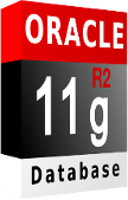
\includegraphics[scale=1]{oracle_11g}
        }
    }
    \begin{lrbox}{\litbox}
        \begin{minipage}{.949\linewidth}
            \smallskip
            }{
            \smallskip
        \end{minipage}
    \end{lrbox}
    \usebox{\litbox}
}

\newenvironment{mssql}[1][\boolean{isTable}]{
    \renewcommand*{\boolparam}{#1}
    \par
    \marginpar{
        \Ifthispageodd{
            \hspace*{0em}
        }
        {
            \hspace*{3em}
        }
        \raisebox{-3\baselineskip}{
            
\includegraphics[scale=1]{ms_sql}
        }
    }
    \begin{lrbox}{\litbox}
        \begin{minipage}{.949\linewidth}
            \smallskip
            }{
            \smallskip
        \end{minipage}
    \end{lrbox}
    \usebox{\litbox}
}

\newenvironment{msoraclesql}[1][\boolean{isTable}]{
    \renewcommand*{\boolparam}{#1}
    \par
    \marginpar{
        \Ifthispageodd{
            \hspace*{0em}
        }
        {
            \hspace*{2.8em}
        }
        \raisebox{-3\baselineskip}{
            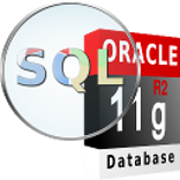
\includegraphics[scale=1]{ms_sql_oracle}
        }
    }
    \begin{lrbox}{\litbox}
        \begin{minipage}{.949\linewidth}
            \smallskip
            }{
            \smallskip
        \end{minipage}
    \end{lrbox}
    \usebox{\litbox}
}
\newenvironment{literaturinternet}{
    \par
    \vspace{.5\baselineskip}
    \marginpar{
        \Ifthispageodd{
            \hspace*{0em}
        }
        {
            \hspace*{2.8em}
        }
        \raisebox{-2\baselineskip}{
            
\includegraphics[scale=1]{globus}
        }
    }
    \begin{lrbox}{\litbox}
        \begin{minipage}{.949\linewidth}
            \smallskip
            \begin{small}
                \begin{itemize}
                    }{
                \end{itemize}
            \end{small}
            \smallskip
        \end{minipage}
    \end{lrbox}
    \fbox{\usebox{\litbox}}
    \par
    \vspace{.5\baselineskip}
    \ignorespacesafterend
}

% \newenvironment{literaturinternet}{
%   \par
%   \leaders\vbox to 2\baselineskip{%

%   }\vskip2\baselineskip
%   \marginpar{\vspace*{-1.5em}\Ifthispageodd{\hspace*{1em}}{\hspace*{3em}}
\includegraphics[scale=1]{globus}}
%   \vspace{-1.5em}
%   \begin{lrbox}{\litbox}
%     \begin{minipage}{.96\linewidth}
%       \begin{small}
%         \begin{itemize}
% }{
%         \end{itemize}
%       \end{small}
%     \end{minipage}
%   \end{lrbox}
%   \fbox{\usebox{\litbox}}
%   \par
%   \addvspace{\baselineskip}
% }

\newcommand{\bild}[3]{
    \begingroup
    \par
    \setcapindent*{-0em}
    \setcapwidth[o]{0.15\linewidth}
    \settoheight{\bildhoehe}{\includegraphics[scale=#3]{#2}}
    \addtolength{\bildhoehe}{-3em}
    \addvspace{\baselineskip}
    \begin{figure}[h!t]
        \begin{captionbeside}{#1}[o][\linewidth][4.3em]*
            \parbox[t][\bildhoehe][b]{0.85\linewidth}{
                \centering\includegraphics[scale=#3]{#2}}
        \end{captionbeside}
        \label{#2}
    \end{figure}
    \par
    \endgroup
}

\newcommand{\identifier}[1]{\textsc{#1}}
\newcommand{\languageorasql}[1]{\lstinline[language=oracle_sql]{#1}}
\newcommand{\languagemssql}[1]{\lstinline[language=ms_sql]{#1}}
\newcommand{\languagerman}[1]{\lstinline[language=rman]{#1}}
\newcommand{\languageplsql}[1]{\lstinline[language=plsql]{#1}}
\newcommand{\languagesqlplus}[1]{\lstinline[language=sqlplus]{#1}}
\newcommand{\languageconfigfile}[1]{\lstinline[language=configfile]{#1}}
\newcommand{\languageexpdpimpdp}[1]{\lstinline[language=expdp_impdp]{#1}}
\newcommand{\languagepowershell}[1]{\lstinline[language=powershell]{#1}}
\newcommand{\oscommand}[1]{\texttt{#1}}
\newcommand{\privileg}[1]{\texttt{#1}}
\newcommand{\parameter}[1]{\MakeLowercase{\textsf{#1}}}

\newcommand{\SELECT}{\languageorasql{SELECT}}
\newcommand{\FROM}{\languageorasql{FROM}}
\newcommand{\WHERE}{\languageorasql{WHERE}}
\newcommand{\GROUPBY}{\languageorasql{GROUP BY}}
\newcommand{\HAVING}{\languageorasql{HAVING}}
\newcommand{\ORDERBY}{\languageorasql{ORDER BY}}
\newcommand{\CHECK}{\languageorasql{CHECK}}
\newcommand{\NOTNULL}{\languageorasql{NOT NULL}}
\newcommand{\UNIQUE}{\languageorasql{UNIQUE}}
\newcommand{\PRIMARYKEY}{\languageorasql{PRIMARY KEY}}
\newcommand{\FOREIGNKEY}{\languageorasql{FOREIGN KEY}}
\newcommand{\INSERT}{\languageorasql{INSERT}}
\newcommand{\UPDATE}{\languageorasql{UPDATE}}
\newcommand{\DELETE}{\languageorasql{DELETE}}
\newcommand{\COMMIT}{\languageorasql{COMMIT}}
\newcommand{\ROLLBACK}{\languageorasql{ROLLBACK}}
\newcommand{\GRANT}{\languageorasql{GRANT}}
\newcommand{\REVOKE}{\languageorasql{REVOKE}}
\newcommand{\DENY}{\languageorasql{DENY}}

\newenvironment{literaturbuch}{
    \marginpar{\vspace{1em}\Ifthispageodd{\hspace*{-4em}}{\hspace*{3em}}\includegraphics[scale=1]{buch}}
    \begin{lrbox}{\litbox}
        \begin{minipage}{.975\linewidth}
            \begin{small}
                \begin{itemize}
                    }{
                \end{itemize}
            \end{small}
        \end{minipage}
    \end{lrbox}
    \par\fbox{\usebox{\litbox}}\par
}

\newcommand{\pk}[1]{\underline{#1}}
\newcommand{\fk}[1]{$\Uparrow$#1$\Uparrow$}
\newcommand{\nn}[1]{#1 [NN]}
\newcommand{\un}[1]{#1 [UN]}

\newcommand{\changefont}[3]{\fontfamily{#1} \fontseries{#2} \fontshape{#3} \selectfont}
\newcommand{\beispiel}[1]{\hyperref[#1]{Beispiel~\ref*{#1}}}
\newcommand{\abschnitt}[1]{\hyperref[#1]{Abschnitt~\ref*{#1}}}
\newcommand{\tabelle}[1]{\hyperref[#1]{Tabelle~\ref*{#1}}}
\newcommand{\abbildung}[1]{\hyperref[#1]{Abbildung~\ref*{#1}}}
\makeatletter
\newcommand{\myhref}[2]{\hyper@linkurl{#2}{#1}}
\makeatother



% KOMAScript guide, p. 66 (3.7 Dokumenttitel)
% Define title and author of this document
\title{Datenbankadministration}
\author{Florian Weidinger}

% KOMAScript guide, p. 271 ff.
\lehead*{}
\rohead*{}
\chead{\leftmark}
\makeatletter
\lofoot*{\normalfont\textbf{\@title{} \@subtitle}}
\makeatother
\rofoot*{\Large\pagemark}
\lefoot*{\Large\pagemark}